\documentclass[12pt]{article}
\usepackage{amsfonts,amssymb,amsmath}
\usepackage{graphicx}
\usepackage{listings}

\begin{document}
\subsection*{P1}
\subsection*{P2}
(2)
Use \textit{drawDE.m} to use subdivision methods that yeilds a polygonal line which approximates \textit{Bezier curve}. \\
For example if we input $n = 5 , \; t = \frac{1}{2}$ and a series points through screen: 
\begin{lstlisting}[language=Matlab]
n = 5; % iterate times 
t = 1/2; % t 
[x,y] = ginput(); %screen input the data 
d = [x,y]; % d(i,:) i = 1,2,.. represents a point 
d = sortrows(d); % sort our data 
b = calculateDE(d, n, t); 
% calculate the points used to draw the curve 
b = sortrows(b); % sort our data 
plot(d(:,1), d(:,2), 'r*'); % draw the input data d
hold on;
plot(b(:,1), b(:,2), 'b-') % draw our curve 
title('Bezier Curve')
\end{lstlisting}
Then we can get the graph: \\
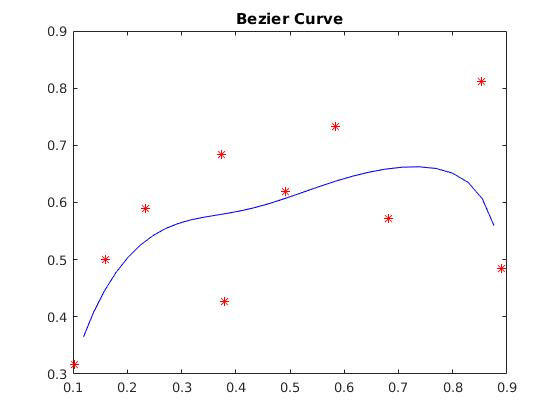
\includegraphics[scale=.5]{npoints}
\end{document}